s\documentclass{beamer}
\usepackage{fontawesome5}
\usetheme{Copenhagen}
\usepackage{german}
\usepackage[ansinew]{inputenc}
\usepackage{pifont}
\usepackage{tikz}
\usetikzlibrary{shapes.geometric, arrows}
\tikzstyle{startstop} = [rectangle, rounded corners, minimum width=1.5cm, minimum height=0.5cm, text centered, draw=black, fill=red!30]
\tikzstyle{process} = [rectangle, minimum width=1.5cm, minimum height=0.5cm, text centered, draw=black, fill=blue!20]
\tikzstyle{processlight} = [rectangle, minimum width=1.5cm, minimum height=0.5cm, text centered, draw=black, fill=blue!10] % hellblau
\tikzstyle{green} = [rectangle, minimum width=1.5cm, minimum height=0.5cm, text centered, draw=black, fill=green!10]
\tikzstyle{arrow} = [thick,->,>=stealth]
\begin{document}
%%%%%%%%%%%%%%%%%%%%%%%%%%%%%%%%%%%%%%%%%%%%%%%%%%%%%%%%%%%%%%%%%%%%%%%%%%%%%%%%%%%%%%
\title{Parametric weather Insurance}   
\author{Kai Frehner and Benjamin Gerber}
\date{Basel, 27th November 2025\\[2mm]
\footnotesize{Smart Contracts and Decentralized Finance}}
\logo{\includegraphics[scale=0.3]{Logo_Basel}}
\begin{frame}
\titlepage
\end{frame}

%%%%%%%%%%%%%%%%%%%%%%%%%%%%%%%%%%%%%%%%%%%%%%%%%%%%%%%%%%%%%%%%%%%%%%%%%%%%%%%%%%%%%%
\begin{frame}{Motivation - Why Parametric Weather Insurance?}

\begin{columns}[T,onlytextwidth]

% LEFT COLUMN ------------------------------------------------------
\begin{column}{0.55\textwidth}
\small
\textbf{Motivation}
\begin{itemize}
    \item Rising frequency of extreme weather events (climate change)
    \item Vulnerability of climate-exposed sectors
    \item Traditional insurance: slow, expensive, data-heavy
    \item Parametric approach: fast, objective, index-based payouts
\end{itemize}
\end{column}

% RIGHT COLUMN -----------------------------------------------------
\begin{column}{0.45\textwidth}
\centering

% --- PHOTO 1: Drought example ---
\includegraphics[width=\linewidth, height=0.27\textheight, keepaspectratio]{drought}\\[4pt]

% --- PHOTO 2: Flooding example ---
\includegraphics[width=\linewidth, height=0.27\textheight, keepaspectratio]{flood}\\[4pt]


\end{column}

\end{columns}
\end{frame}

%%%%%%%%%%%%%%%%%%%%%%%%%%%%%%%%%%%%%%%%%%%%%%%%%%%%%%%%%%%%%%%%%%%%%%%%%%%%%%%%%%%%%%
\begin{frame}
\frametitle{Gliederung}
\tableofcontents
\end{frame}

%%%%%%%%%%%%%%%%%%%%%%%%%%%%%%%%%%%%%%%%%%%%%%%%%%%%%%%%%%%%%%%%%%%%%%%%%%%%%%%%%%%%%%
\section{Parametric Insurance}
\subsection{Parametric vs Traditional Insurance}
\begin{frame}{Parametric vs. Traditional Insurance}
\begin{columns}[T,onlytextwidth]

% LEFT COLUMN ------------------------------------------------------
\begin{column}{0.48\textwidth}
\textbf{Parametric Insurance}
\begin{itemize}
    \item[\faCloudSun] Payout based on weather index
    \item[\faBolt] Fast and transparent
    \item[\faCoins] Lower administrative costs
    \item[\faExclamationCircle] Less moral hazard
    \item[\faExclamationTriangle] Basis risk may exist
    \item[\faChartLine] Scalable
\end{itemize}
\end{column}

% RIGHT COLUMN -----------------------------------------------------
\begin{column}{0.48\textwidth}
\textbf{Traditional Insurance}
\begin{itemize}
    \item[\faFile] Payout based on actual loss
    \item[\faClock] Slow, requires assessment
    \item[\faMoneyBillWave] Higher administrative costs
    \item[\faUserSecret] Possible moral hazard
    \item[\faCheckCircle] Payout matches loss
    \item[\faCogs] Less scalable
\end{itemize}
\end{column}

\end{columns}
\end{frame}


%%%%%%%%%%%%%%%%%%%%%%%%%%%%%%%%%%%%%%%%%%%%%%%%%%%%%%%%%%%%%%%%%%%%%%%%%%%%%%%%%%%%%%
\subsection{Wetterheld - Bad weather Insurance}
\begin{frame}{Parasurance: Parametric Bad-Weather Coverage}
\scriptsize % ca. 75% Schriftgröße

\begin{columns}[T,onlytextwidth]

% LEFT COLUMN ------------------------------------------------------
\begin{column}{0.75\textwidth}
\textbf{Overview:} Multi-parametric travel insurance by Baloise, with Wetterheld monitoring weather.

\begin{itemize}
    \item \textbf{Trigger:} Daily precipitation $>$ 2.9 mm (rain, snow, hail) between 10 a.m. -- 6 p.m.
    \item \textbf{Geography:} GPS-verified European destinations; coverage only at reported location
    \item \textbf{Time restriction:} Must be purchased at least 14 days before trip; trips 2--92 days
    \item \textbf{Deductible days:} First days may be excluded depending on region and season
    \item \textbf{Coverage:} Part of Parasurance; includes flight delay, luggage delay, optional motor liability
    \item \textbf{Monitoring:} Wetterheld uses Meteostat weather data to verify triggers
\end{itemize}
\end{column}

% RIGHT COLUMN -----------------------------------------------------
\begin{column}{0.25\textwidth}
\centering
\includegraphics[width=0.9 \linewidth,height=0.8\textheight,keepaspectratio]{plane.jpg} % Bilddatei mit Endung
\end{column}

\end{columns}
\end{frame}
%%%%%%%%%%%%%%%%%%%%%%%%%%%%%%%%%%%%%%%%%%%%%%%%%%%%%%%%%%%%%%%%%%%%%%%%%%%%%%%%%%%%%%
\section{Implementation via Smart Contract} 
\subsection{Design of a Parametric Travel Insurance}

\begin{frame}{Parametric Weather Insurance: Process Flow}
\tiny % Schrift auf ca. 50%

\centering
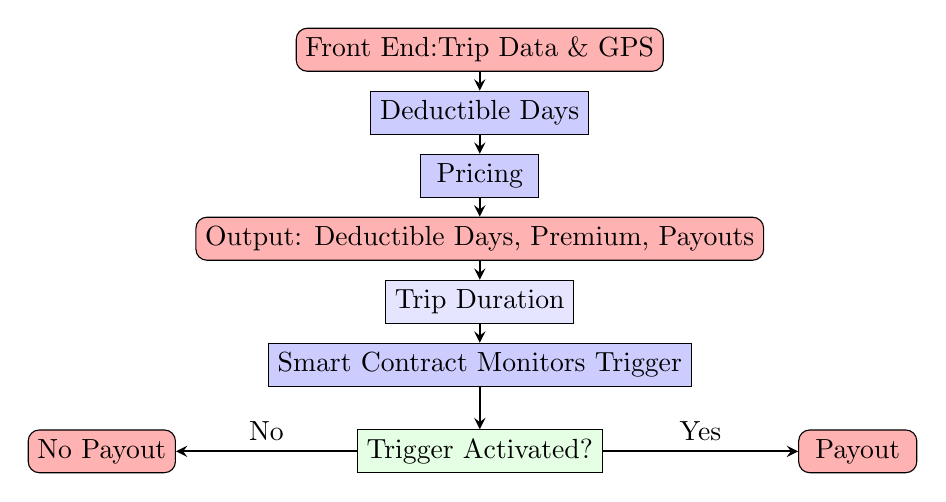
\begin{tikzpicture}[node distance=0.8cm]

% Nodes
\node (frontend) [startstop] {Front End:\\ Trip Data \& GPS};
\node (deductible) [process, below of=frontend] {Deductible Days};
\node (pricing) [process, below of=deductible] {Pricing};
\node (output) [startstop, below of=pricing] {Output: Deductible Days, Premium, Payouts};
\node (trip) [processlight, below of=output] {Trip Duration}; % hellblau
\node (smartcontract) [process, below of=trip] {Smart Contract Monitors Trigger};
\node (trigger) [green, below of=smartcontract, yshift=-0.3cm] {Trigger Activated?};
\node (pay) [startstop, right of=trigger, xshift=4cm] {Payout};
\node (no_pay) [startstop, left of=trigger, xshift=-4cm] {No Payout};

% Arrows
\draw [arrow] (frontend) -- (deductible);
\draw [arrow] (deductible) -- (pricing);
\draw [arrow] (pricing) -- (output);
\draw [arrow] (output) -- (trip);
\draw [arrow] (trip) -- (smartcontract);
\draw [arrow] (smartcontract) -- (trigger);
\draw [arrow] (trigger.east) -- (pay.west) node[midway, above]{Yes};
\draw [arrow] (trigger.west) -- (no_pay.east) node[midway, above]{No};

\end{tikzpicture}
\end{frame}
%%%%%%%%%%%%%%%%%%%%%%%%%%%%%%%%%%%%%%%%%%%%%%%%%%%%%%%%%%%%%%%%%%%%%%%%%%%%%%%%%%%%%%
\subsection{Incorporating local weather conditions}
\begin{frame}{Deductible Days: Methodology}
\footnotesize % etwas kleinere Schrift für mehr Übersicht

\begin{columns}[T,onlytextwidth]
% LEFT IMAGE
\begin{column}{0.48\textwidth}
\centering
\includegraphics[width=\linewidth,height=0.4\textheight,keepaspectratio]{spain} % Bild Spanien
\captionof{Spain: low rainfall}
\end{column}

% RIGHT IMAGE
\begin{column}{0.48\textwidth}
\centering
\includegraphics[width=\linewidth,height=0.4\textheight,keepaspectratio]{england} % Bild England
\captionof{England: frequent rain}
\end{column}
\end{columns}

\vspace{0.3cm}

\begin{itemize}
    \item Data from \textbf{European Climate Assessment \& Dataset (ECA\&D)} project
    \item 3.1 GB daily precipitation data since early 20th century
    \item $>$16,000 weather stations across Europe
\end{itemize}

\end{frame}
\begin{frame}{Deriving the Five Risk Categories (Using R)}
\footnotesize

\begin{itemize}
    \item To reduce computation time and storage, we randomly selected \textbf{1,000 weather stations}
    \item For each station and each calendar year: count all days with \(\ge 2.9\) mm precipitation
    \item Plot the histogram of annual rainy days across all sampled stations
    \item Compute the \textbf{20\% quantile steps} \ five thresholds
    \item This yields the five \textbf{risk categories A $-$ E}
\end{itemize}

\vspace{0.2cm}

\begin{columns}[T,onlytextwidth]  % <-- T = top-aligned

% HISTOGRAM ---------------------------------
\begin{column}{0.48\textwidth}
\centering
\includegraphics[width=\linewidth,height=0.35\textheight,keepaspectratio]{hist}

\end{column}

% MAP WITH STATIONS -------------------------
\begin{column}{0.48\textwidth}
\centering
\includegraphics[width=\linewidth,height=0.35\textheight,keepaspectratio]{weatherstations}

\end{column}

\end{columns}

\end{frame}
%%%%%%%%%%%%%%%%%%%%%%%%%%%%%%%%%%%%%%%%%%%%%%%%%%%%%%%%%%%%%%%%%%%%%%%%%%%%%%%%%%%%%%
\subsection{Pricing} 
\begin{frame}
\frametitle{5. Folientitel Hauptteil} 
\end{frame}

%%%%%%%%%%%%%%%%%%%%%%%%%%%%%%%%%%%%%%%%%%%%%%%%%%%%%%%%%%%%%%%%%%%%%%%%%%%%%%%%%%%%%%
\subsection{Implementation with Solidity}
\begin{frame}
\frametitle{6. Folientitel Hauptteil}
\end{frame}
%%%%%%%%%%%%%%%%%%%%%%%%%%%%%%%%%%%%%%%%%%%%%%%%%%%%%%%%%%%%%%%%%%%%%%%%%%%%%%%%%%%%%%
\section{Example case - Trip to Berlin} 
\begin{frame}{Example: Trip to Berlin}
\footnotesize

\begin{columns}[T,onlytextwidth]

% LEFT COLUMN -------------------------------------------------
\begin{column}{0.60\textwidth}

\begin{itemize}
    \item Trip duration: \textbf{12 Jan 2026$-$23 Jan 2026} (12 days)
    \item Berlin has on average \textbf{65 rainy days/year} with precipitation $\ge 2.9$ mm
    \item $\Rightarrow$ Risk category: \textbf{C}
    \item Deductible days: $\text{round}(12 \times 0.3) = 4$
    \item Payout is triggered starting from the \textbf{5th rainy day}
    \item Coverage amount = \textbf{50 EUR/day} (Assumption)
    \item Premium:  
    \[
        50 EUR \times (12 - 4) \times 0.3 \times 1.1
        = \textbf{132 EUR}
    \]
\end{itemize}

\end{column}

% RIGHT COLUMN ------------------------------------------------
\begin{column}{0.37\textwidth}
\centering
\includegraphics[width=\linewidth,height=0.55\textheight,keepaspectratio]{berlin}
\end{column}

\end{columns}

\end{frame}
%%%%%%%%%%%%%%%%%%%%%%%%%%%%%%%%%%%%%%%%%%%%%%%%%%%%%%%%%%%%%%%%%%%%%%%%%%%%%%%%%%%%%%
\section{Conclusion} 
\begin{frame}{Key Findings: Blockchain-based Parametric Insurance}
\begin{itemize}
    \item Parametric insurance enables fast, transparent, and objective payouts.
    \item Smart contracts enhance efficiency, immutability, and automated evaluation.
    \item Ethereum Sepolia prototype demonstrates feasibility with deductible logic, regional risk factors, and automatic payouts.
    \item Reliance on oracles introduces risks: faulty, delayed, or manipulated data can affect payouts.
    \item Oracle risks can be mitigated via decentralized network and multi-source aggregation
    \item Overall: blockchain-based parametric insurance can increase transparency, speed, and scalability as oracle systems mature.
\end{itemize}
\end{frame}

%%%%%%%%%%%%%%%%%%%%%%%%%%%%%%%%%%%%%%%%%%%%%%%%%%%%%%%%%%%%%%%%%%%%%%%%%%%%%%%%%%%%%%
\begin{frame}
\frametitle{Thank you}
\begin{center}
\LARGE{\textcolor{blue}{Thank you for your attention!\\[5mm]
We're happy to answer any questions}}
~\\[6mm]
\small{{\\[5mm]
\ding{45} kai.frehner@stud.unibas.ch\\
\ding{45} benjamin.gerber@stud.unibas.ch}}

\end{center}
\end{frame}

%%%%%%%%%%%%%%%%%%%%%%%%%%%%%%%%%%%%%%%%%%%%%%%%%%%%%%%%%%%%%%%%%%%%%%%%%%%%%%%%%%%%%%
\section{References}
\begin{frame}
\frametitle{Literaturliste}
\begin{thebibliography}{9}
\bibitem[Beamerpaket]{paket}
\emph{Beamer Paket}. \text{http://latex-beamer.sourceforge.net/}
\bibitem[Beamerdokumentation]{doku}
\emph{User's Guide to the Beamer} 
\end{thebibliography}
\end{frame}

%%%%%%%%%%%%%%%%%%%%%%%%%%%%%%%%%%%%%%%%%%%%%%%%%%%%%%%%%%%%%%%%%%%%%%%%%%%%%%%%%%%%%%

\end{document}

